\documentclass[10pt]{beamer}
\usetheme{Singapore}
\usepackage[utf8]{inputenc}
\usepackage{amsmath}
\usepackage{amsfonts}
\usepackage{amssymb}
%\author{}
%\title{}
%\setbeamercovered{transparent} 
%\setbeamertemplate{navigation symbols}{} 
%\logo{} 
%\institute{} 
%\date{} 
%\subject{} 
\title{Predicción de la población para los próximos cuatro años}
\subtitle{Test de programación – Jr. Data Engineer - \textbf{Ventagium}}
\author{F.E. Charry-Pastrana}
%\institute{Overleaf}
\date{2021.07.13}

\usepackage{ragged2e}

\apptocmd{\frame}{}{\justifying}{} % Allow optional arguments after frame.

\begin{document}

\begin{frame}
\titlepage
\end{frame}

%\begin{frame}
%\tableofcontents
%\end{frame}

\begin{frame}{Resultados}
\begin{figure}
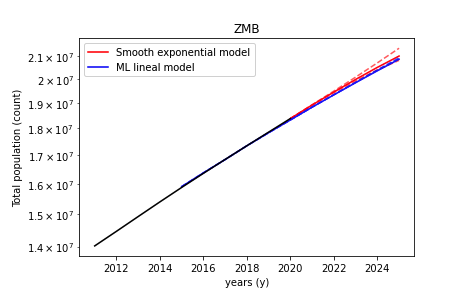
\includegraphics[scale=0.3]{img/1.png}
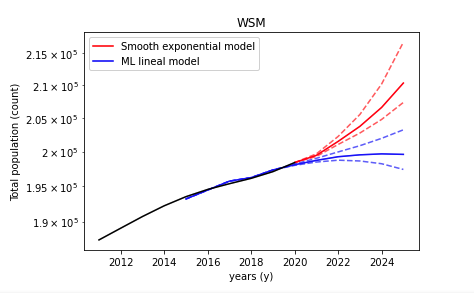
\includegraphics[scale=0.3]{img/2.png}
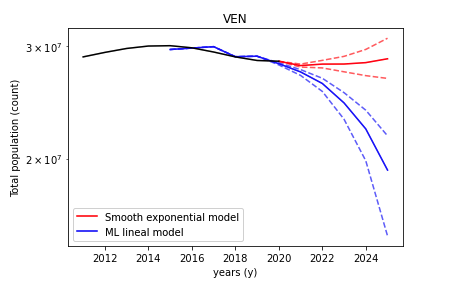
\includegraphics[scale=0.3]{img/3.png}
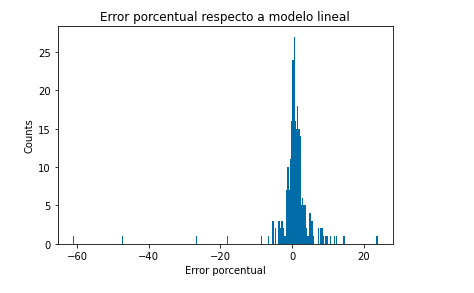
\includegraphics[scale=0.3]{img/4.png}
\end{figure}
\end{frame}

\begin{frame}{Exploración de datos}
\begin{columns}
\begin{column}{0.38\textwidth}  %%<--- here
    \begin{figure}
    \centering
     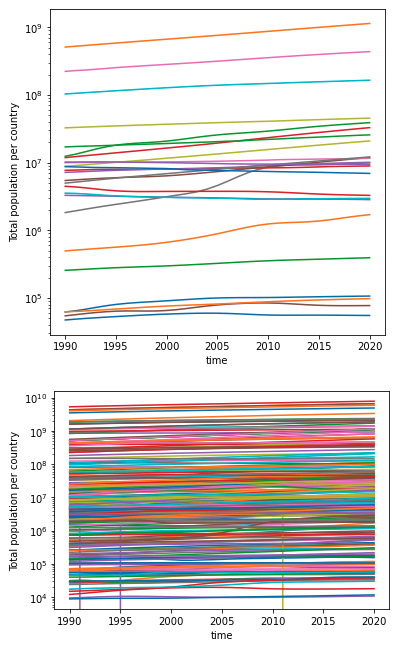
\includegraphics[scale=0.27]{img/5.png}
     \end{figure}
\begin{equation*}
\log(P(t)) = A\, t + B
\end{equation*}
\end{column}
\begin{column}{0.65\textwidth}
\justifying Población $P$ depende de tiempo $t$,  natalidad $n$, mortalidad $d$ y migración $m$. 
\begin{align*}
P(t) &\propto f(t, n, d,m), \\
&\propto f(t, n(t), d(t),m(t)),  \\
 &\propto f(t, n(t), d(t)).
\end{align*}
\begin{figure}
\centering
     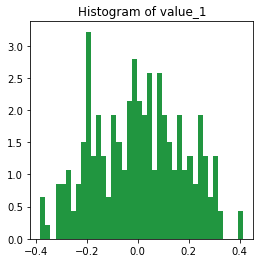
\includegraphics[scale=0.3]{img/6.png}
     \caption{Correlación entre $P(t)$ y $m(t)$}
     \end{figure}
\end{column}
\end{columns}
\end{frame}

\begin{frame}{Modelos inicial}
$P(t)$ depende únicamente del tiempo $t$ de forma exponencial, 
\begin{figure}
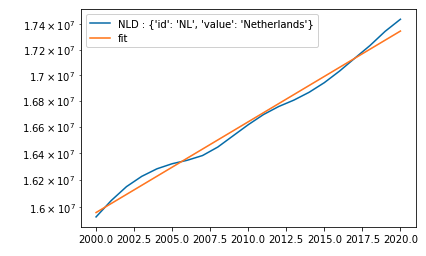
\includegraphics[scale=0.35]{img/7.png}
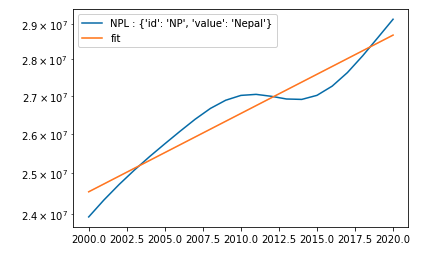
\includegraphics[scale=0.35]{img/8.png}
\end{figure}
sin embargo, el modelo no captura las variaciones de los últimos años
\end{frame}

\begin{frame}[fragile]{Modelos exponencial con corrección de los últimos años}
\begin{equation*}
P(t+1) = A\,\exp(B\,t) + \overline{\delta},
\end{equation*}
\begin{equation*}
\delta = P(t) - P_\text{real}(t) 
\end{equation*}
\begin{verbatim}
y_predict = exp(x[j+4], parameters) - mean(delta[-2:])
delta = y_predict - y[j+4]
\end{verbatim}
\begin{figure}
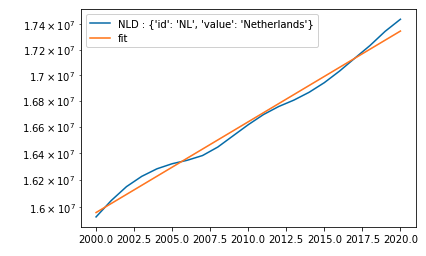
\includegraphics[scale=0.35]{img/7.png}
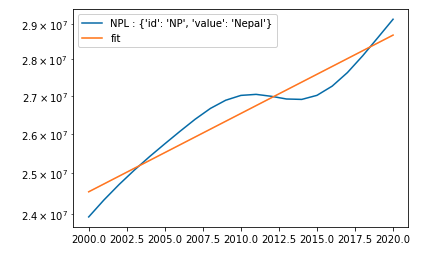
\includegraphics[scale=0.35]{img/8.png}
\end{figure}
\end{frame}


\end{document}